% Options for packages loaded elsewhere
\PassOptionsToPackage{unicode}{hyperref}
\PassOptionsToPackage{hyphens}{url}
\PassOptionsToPackage{dvipsnames,svgnames,x11names}{xcolor}
%
\documentclass[
  12pt,
  letterpaper,
  DIV=11,
  numbers=noendperiod]{scrartcl}

\usepackage{amsmath,amssymb}
\usepackage{iftex}
\ifPDFTeX
  \usepackage[T1]{fontenc}
  \usepackage[utf8]{inputenc}
  \usepackage{textcomp} % provide euro and other symbols
\else % if luatex or xetex
  \usepackage{unicode-math}
  \defaultfontfeatures{Scale=MatchLowercase}
  \defaultfontfeatures[\rmfamily]{Ligatures=TeX,Scale=1}
\fi
\usepackage{lmodern}
\ifPDFTeX\else  
    % xetex/luatex font selection
\fi
% Use upquote if available, for straight quotes in verbatim environments
\IfFileExists{upquote.sty}{\usepackage{upquote}}{}
\IfFileExists{microtype.sty}{% use microtype if available
  \usepackage[]{microtype}
  \UseMicrotypeSet[protrusion]{basicmath} % disable protrusion for tt fonts
}{}
\makeatletter
\@ifundefined{KOMAClassName}{% if non-KOMA class
  \IfFileExists{parskip.sty}{%
    \usepackage{parskip}
  }{% else
    \setlength{\parindent}{0pt}
    \setlength{\parskip}{6pt plus 2pt minus 1pt}}
}{% if KOMA class
  \KOMAoptions{parskip=half}}
\makeatother
\usepackage{xcolor}
\setlength{\emergencystretch}{3em} % prevent overfull lines
\setcounter{secnumdepth}{-\maxdimen} % remove section numbering
% Make \paragraph and \subparagraph free-standing
\makeatletter
\ifx\paragraph\undefined\else
  \let\oldparagraph\paragraph
  \renewcommand{\paragraph}{
    \@ifstar
      \xxxParagraphStar
      \xxxParagraphNoStar
  }
  \newcommand{\xxxParagraphStar}[1]{\oldparagraph*{#1}\mbox{}}
  \newcommand{\xxxParagraphNoStar}[1]{\oldparagraph{#1}\mbox{}}
\fi
\ifx\subparagraph\undefined\else
  \let\oldsubparagraph\subparagraph
  \renewcommand{\subparagraph}{
    \@ifstar
      \xxxSubParagraphStar
      \xxxSubParagraphNoStar
  }
  \newcommand{\xxxSubParagraphStar}[1]{\oldsubparagraph*{#1}\mbox{}}
  \newcommand{\xxxSubParagraphNoStar}[1]{\oldsubparagraph{#1}\mbox{}}
\fi
\makeatother


\providecommand{\tightlist}{%
  \setlength{\itemsep}{0pt}\setlength{\parskip}{0pt}}\usepackage{longtable,booktabs,array}
\usepackage{calc} % for calculating minipage widths
% Correct order of tables after \paragraph or \subparagraph
\usepackage{etoolbox}
\makeatletter
\patchcmd\longtable{\par}{\if@noskipsec\mbox{}\fi\par}{}{}
\makeatother
% Allow footnotes in longtable head/foot
\IfFileExists{footnotehyper.sty}{\usepackage{footnotehyper}}{\usepackage{footnote}}
\makesavenoteenv{longtable}
\usepackage{graphicx}
\makeatletter
\def\maxwidth{\ifdim\Gin@nat@width>\linewidth\linewidth\else\Gin@nat@width\fi}
\def\maxheight{\ifdim\Gin@nat@height>\textheight\textheight\else\Gin@nat@height\fi}
\makeatother
% Scale images if necessary, so that they will not overflow the page
% margins by default, and it is still possible to overwrite the defaults
% using explicit options in \includegraphics[width, height, ...]{}
\setkeys{Gin}{width=\maxwidth,height=\maxheight,keepaspectratio}
% Set default figure placement to htbp
\makeatletter
\def\fps@figure{htbp}
\makeatother

\usepackage{booktabs}
\usepackage{float}
\floatplacement{table}{H}
\usepackage{setspace}
\onehalfspacing
\usepackage{geometry}
\geometry{left=1in, right=1in, top=1in, bottom=1in}
\KOMAoption{captions}{tableheading}
\usepackage{amsmath}
\usepackage{amssymb}
\usepackage{graphicx}
\usepackage{geometry}
\makeatletter
\@ifpackageloaded{caption}{}{\usepackage{caption}}
\AtBeginDocument{%
\ifdefined\contentsname
  \renewcommand*\contentsname{Table of contents}
\else
  \newcommand\contentsname{Table of contents}
\fi
\ifdefined\listfigurename
  \renewcommand*\listfigurename{List of Figures}
\else
  \newcommand\listfigurename{List of Figures}
\fi
\ifdefined\listtablename
  \renewcommand*\listtablename{List of Tables}
\else
  \newcommand\listtablename{List of Tables}
\fi
\ifdefined\figurename
  \renewcommand*\figurename{Figure}
\else
  \newcommand\figurename{Figure}
\fi
\ifdefined\tablename
  \renewcommand*\tablename{Table}
\else
  \newcommand\tablename{Table}
\fi
}
\@ifpackageloaded{float}{}{\usepackage{float}}
\floatstyle{ruled}
\@ifundefined{c@chapter}{\newfloat{codelisting}{h}{lop}}{\newfloat{codelisting}{h}{lop}[chapter]}
\floatname{codelisting}{Listing}
\newcommand*\listoflistings{\listof{codelisting}{List of Listings}}
\makeatother
\makeatletter
\makeatother
\makeatletter
\@ifpackageloaded{caption}{}{\usepackage{caption}}
\@ifpackageloaded{subcaption}{}{\usepackage{subcaption}}
\makeatother

\ifLuaTeX
  \usepackage{selnolig}  % disable illegal ligatures
\fi
\usepackage{bookmark}

\IfFileExists{xurl.sty}{\usepackage{xurl}}{} % add URL line breaks if available
\urlstyle{same} % disable monospaced font for URLs
\hypersetup{
  pdftitle={Analysis of Cancer Data},
  pdfauthor={Group\_37},
  colorlinks=true,
  linkcolor={blue},
  filecolor={Maroon},
  citecolor={Blue},
  urlcolor={Blue},
  pdfcreator={LaTeX via pandoc}}


\title{Analysis of Cancer Data}
\author{Group\_37}
\date{}

\begin{document}
\maketitle


\subsection{Data sets created}\label{data-sets-created}

\section{Introduction}\label{introduction}

Modern mass spectrometry collects thousands of molecular features, but
analyzing such high-dimensional data is challenging. Identifying key
patterns can aid early diagnosis and improve treatment.

To explore the question, the Arcene dataset will be divided into a
training set and a test set. A unique training set containing 100
samples with 5,000 randomly selected features. A fixed test set (100
samples with all 10,000 features) will be used for model evaluation. The
study will employ various classification techniques to assess their
accuracy in distinguishing between cancerous and normal tissue samples.
Through the model analysis, to explore the following research questions:

\begin{itemize}
\item
  \textbf{Primary research question}: Can biochemical features
  accurately distinguish between cancerous and normal tissue samples?
\item
  \textbf{Secondary research question}: Compare the results of different
  classification models to find out a best classification model.
\end{itemize}

\section{Data Processing}\label{data-processing}

\subsection{Initial rejection of potential
probes}\label{initial-rejection-of-potential-probes}

Based on the dataset description, we performed an initial feature
selection process to reduce the dimensionality of the data and eliminate
variables that may not provide meaningful insights for the model. We
focused on removing features with extremely low variance, as these are
typically considered to be probes or noise sequences that do not
contribute valuable information for predictive modeling. Such features
often show minimal variability across observations and do not offer
distinguishing power for classification or regression tasks. By removing
these low-variance features, we reduced the data dimensionality, which
facilitates more efficient analysis and model training, and helps to
prevent overfitting by removing redundant or irrelevant information.
This step is essential for improving the overall performance and
interpretability of the model.

\begin{figure}

\centering{

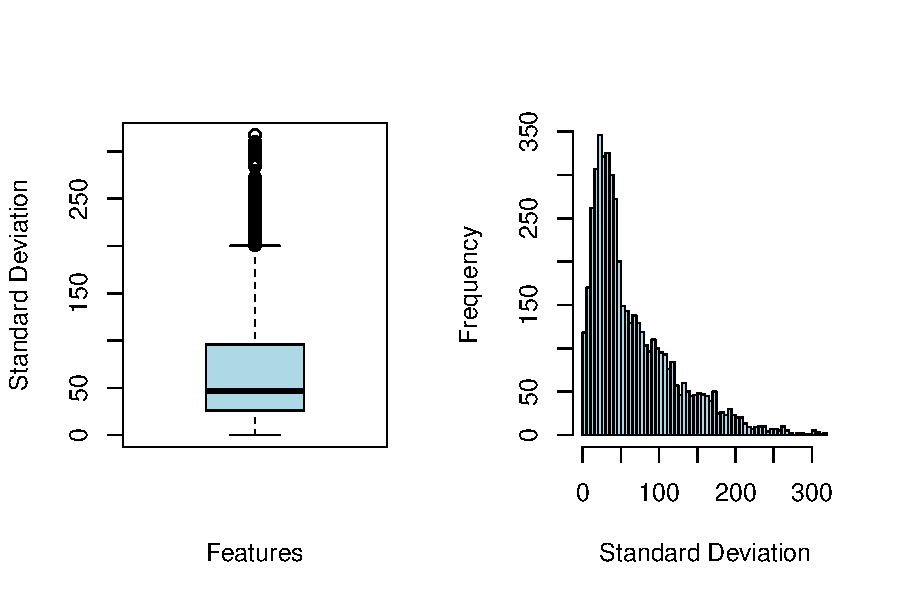
\includegraphics{me_files/figure-pdf/fig-init1-1.pdf}

}

\caption{\label{fig-init1}Variable Standard Deviation Distribution}

\end{figure}%

\subsection{Data Dimension Reduction
Processing}\label{data-dimension-reduction-processing}

PCA was further applied to reduce the dimensionality of the data. The
Kaiser criterion and the cumulative variance contribution ratio were
used to select the effective principal components. Based on these
criteria, the original dataset was updated, leading to a significant
reduction in its dimensionality.

\section{Formal data analysis}\label{formal-data-analysis}

\subsection{Tree-based methods}\label{tree-based-methods}

\subsubsection{Classification Tree}\label{classification-tree}

Classification Tree partition the feature space into a number of
disjoint and non-overlapping regions. And predict the class of a given
observation as the most commonly occurring class of training
observations is the region to which it belongs.

\begin{figure}

\centering{

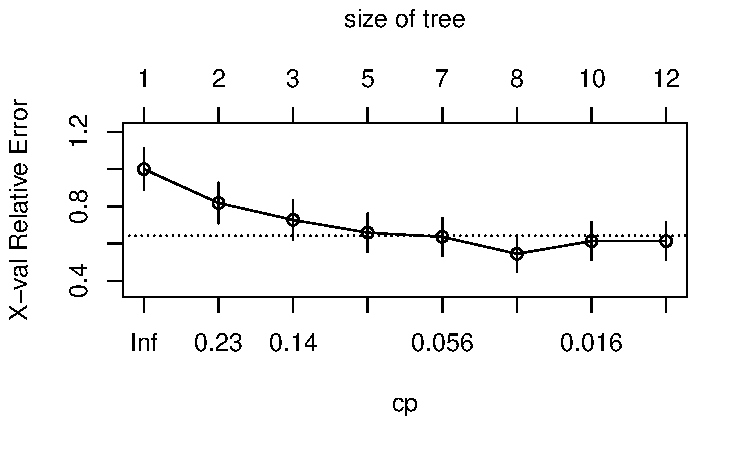
\includegraphics{me_files/figure-pdf/fig-tree1-1.pdf}

}

\caption{\label{fig-tree1}Xerror vs CP}

\end{figure}%

The pruning process is based on the complexity parameter (cp) selection.
The optimal cp is chosen as the largest value within the range where the
cross-validation error remains within one standard deviation of the
minimum error. Based on this criterion, a cp of 0.032 is selected to
prune the new tree.

\begin{figure}

\centering{

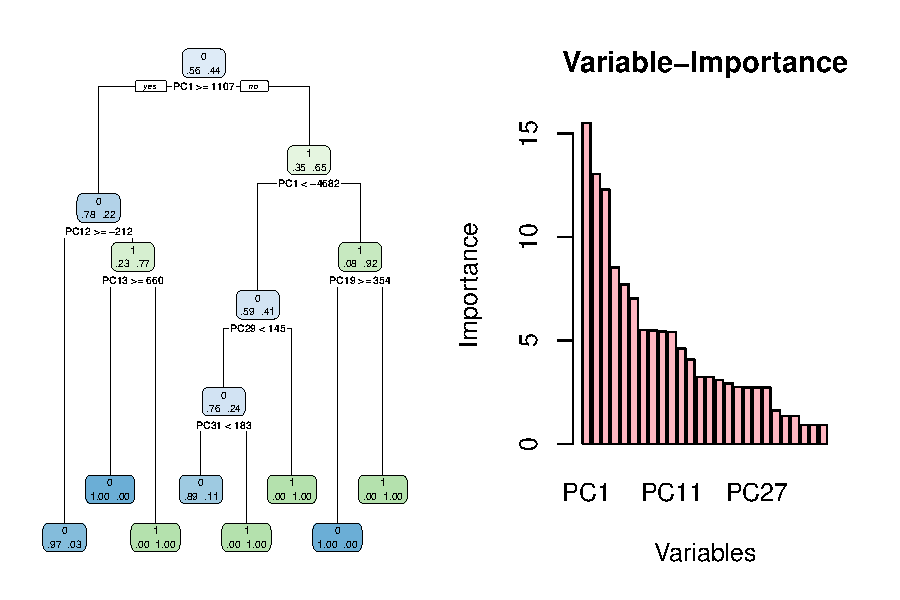
\includegraphics{me_files/figure-pdf/fig-tree2-1.pdf}

}

\caption{\label{fig-tree2}Pruned Classification Tree (cp=0.032)}

\end{figure}%

The classification tree also highlights the importance of variables,
showing that PC1 is the most significant, followed by PC12 and PC2.
Variables like PC18, PC13, PC21, and PC24 are considered less important.

The test accuracy is 0.68, indicating poor performance. While the
classification tree has some predictive ability, its overall
effectiveness is limited.

\subsubsection{Bagging Tree}\label{bagging-tree}

The core idea of bagging is to repeatedly draw samples from the original
dataset and build a classification tree on each bootstrapped sample. For
each test observation, the class predicted by each tree is recorded. The
final prediction is determined by a majority vote, where the class that
appears most frequently across all predictions becomes the overall
predicted class. To select the minimum number of trees that stabilize
the OOB error, the model was trained with different numbers of trees,
and the OOB error was monitored. Once the error stabilized, the smallest
number of trees that achieved this stabilization was chosen to build the
final Bagging Tree model.

\begin{figure}

\centering{

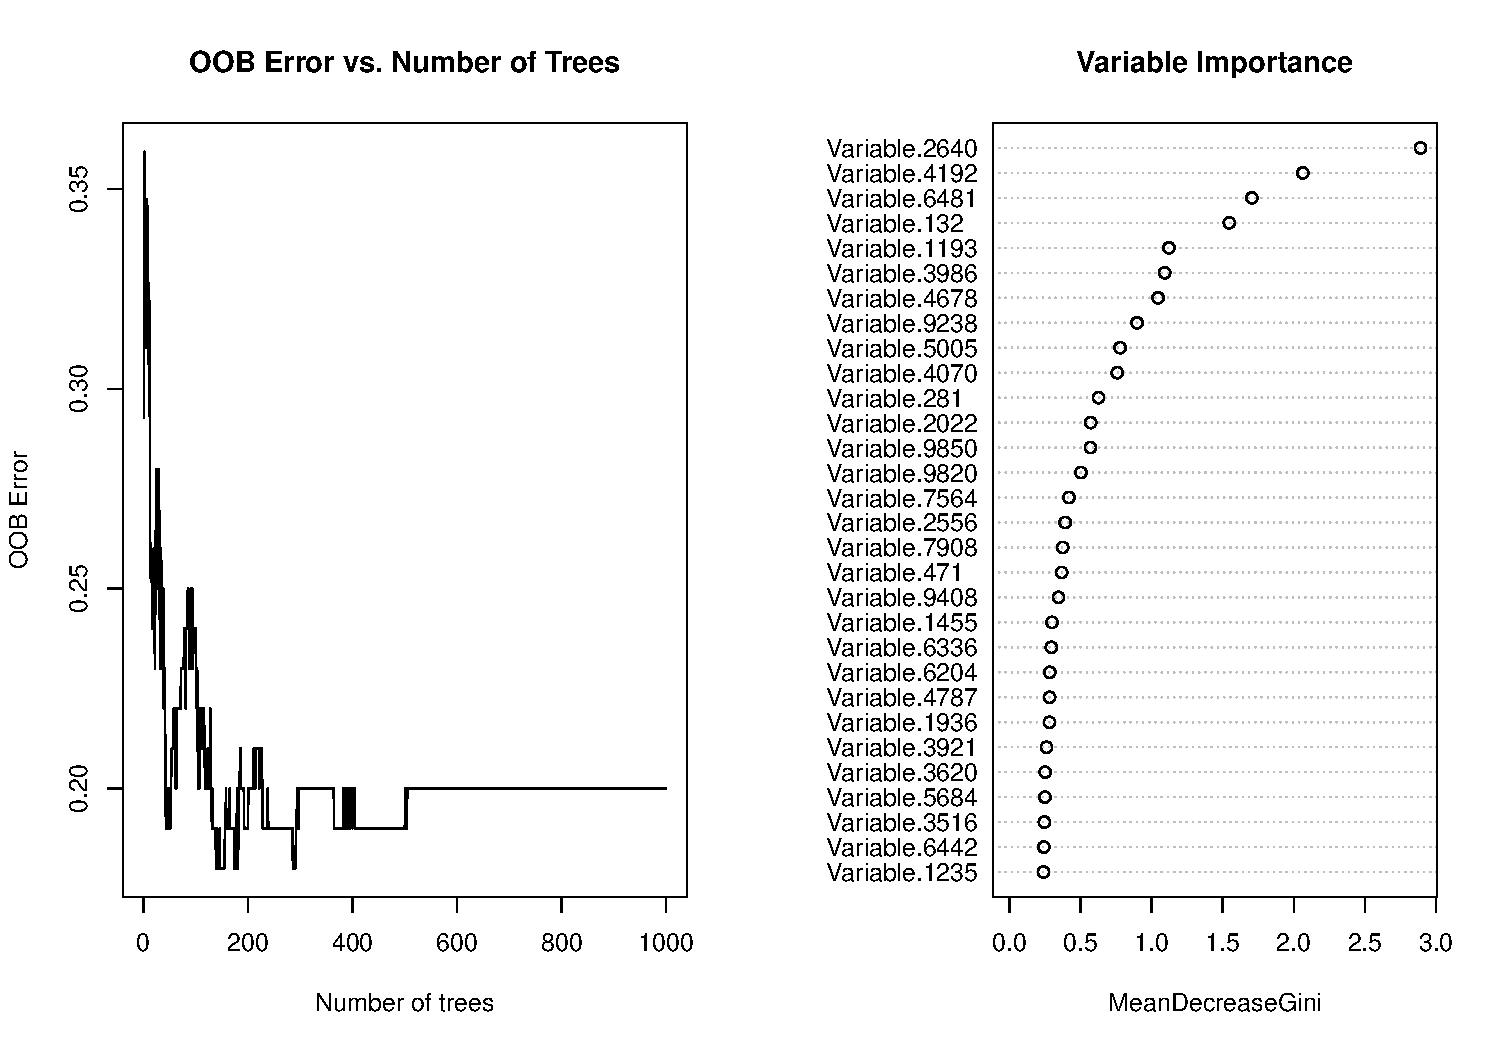
\includegraphics{me_files/figure-pdf/fig-tree5-1.pdf}

}

\caption{\label{fig-tree5}Model Performance}

\end{figure}%

According to the Bagging Tree, Variable.2640 is the most important
factor, followed by Variable.4192 and Variable.6481, Variable.132 and
Variable.1193, Variable.6442 and Variable.1235 are relatively
unimportant.The Accuracy of test is 0.79, which is good. Showing the
Bagging Tree has good classification ability.

{[}1{]} ``Accuracy: 0.79'' Actual Predicted 0 1 0 45 10 1 11 34 {[}1{]}
``AUC: 0.895292207792208''

\subsubsection{Random Forests}\label{random-forests}

Random forests enhance Bagging Tree by reducing the correlation between
individual trees. By randomly excluding a subset of variables at each
split, the trees become more diverse, leading to more stable and
reliable predictions.

OBB(out of bag)

\begin{figure}

\centering{

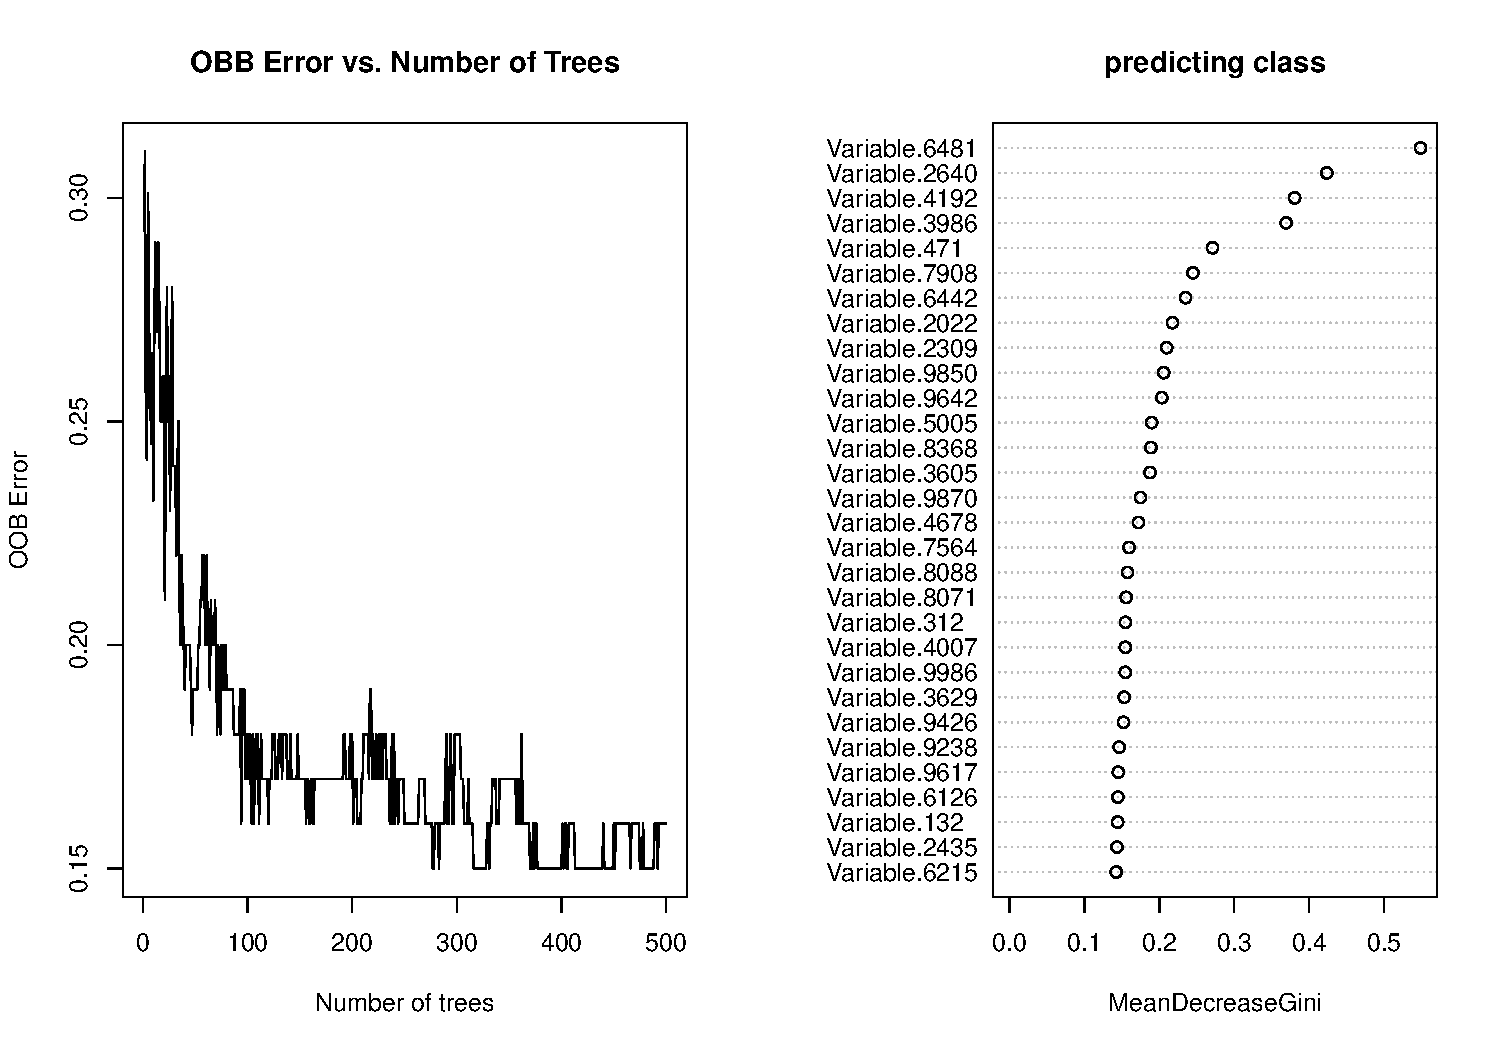
\includegraphics{me_files/figure-pdf/fig-tree8-1.pdf}

}

\caption{\label{fig-tree8}Model Performance}

\end{figure}%

According to the random forests, Variable.2640 and Variable.4192, which
were also important in the Bagging model, remain influential.

\begin{figure}

\centering{

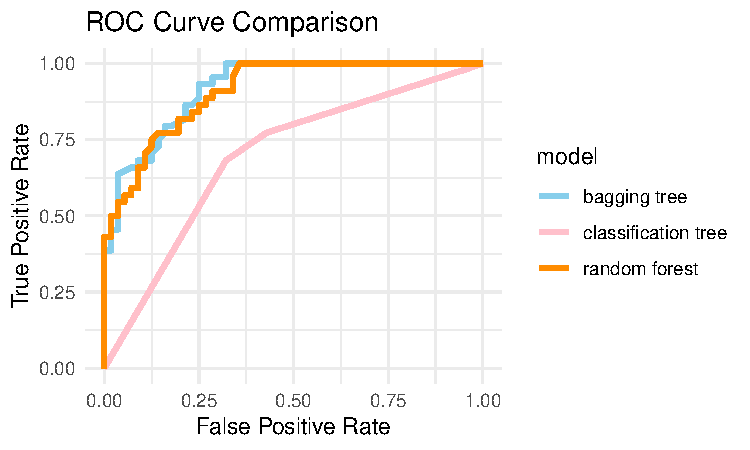
\includegraphics{me_files/figure-pdf/fig-tree10-1.pdf}

}

\caption{\label{fig-tree10}ROC Plot Compare}

\end{figure}%

The ROC comparison shows that the AUC values for the classification
tree, bagging tree, and random forest are 0.6936, 0.8953, and 0.9111,
respectively. Since the random forest achieves the highest AUC, it
demonstrates the best predictive performance among the three models.

\subsection{Discriminant Analysis}\label{discriminant-analysis}

\subsubsection{Test of boxm}\label{test-of-boxm}

The Box's M-test for homogeneity of covariance matrices was performed,
with the results showing a Chi-Square value of 576.49 and degrees of
freedom (df) equal to 171. The p-value was extremely small (\textless{}
2.2e-16), indicating that the assumption of homogeneity of covariance
matrices is violated. However, I still proceeded with LDA as a
comparison method.

Next, the Shapiro-Wilk normality test was conducted for each feature,
and the Bonferroni correction was applied to adjust for multiple
comparisons. A total of 5 features failed the normality test after the
correction, meaning they do not follow a normal distribution.

Two classification models, Linear Discriminant Analysis (LDA) and
Quadratic Discriminant Analysis (QDA), were then applied to the data.
For LDA, the accuracy was 73\%, with a confusion matrix showing 45 true
negatives, 28 true positives, 11 false positives, and 16 false
negatives. For QDA, the accuracy improved to 79\%, with a confusion
matrix showing 48 true negatives, 31 true positives, 8 false positives,
and 13 false negatives. Finally, ROC curves were plotted for both LDA
and QDA. The AUC (Area Under the Curve) values were printed on the
plots, providing a visual representation of the models' performance. The
AUC for QDA was superior to that of LDA, indicating that QDA had better
discriminatory power in distinguishing between the two classes.

\begin{figure}[H]

{\centering 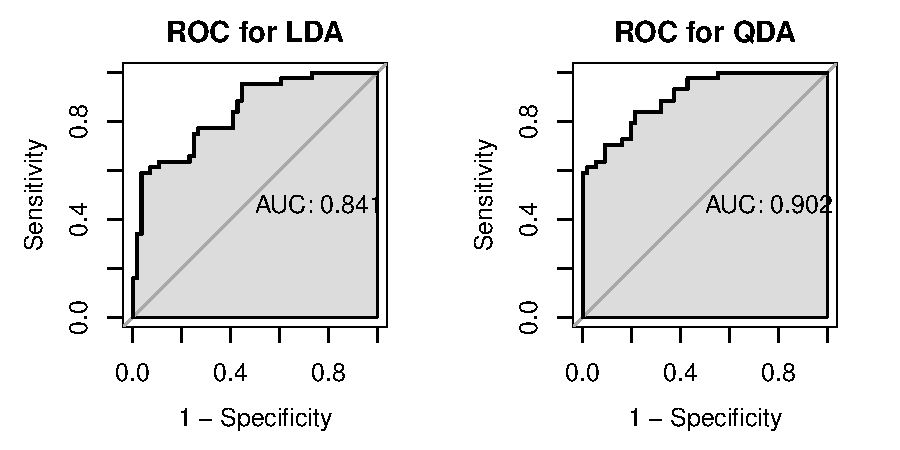
\includegraphics{me_files/figure-pdf/ROC of LDA and QDA-1.pdf}

}

\caption{ROC}

\end{figure}%

The histograms show that both LDA and QDA assign most observations with
probabilities close to 0 or 1, indicating high confidence in their
classifications. This could suggest that the models are performing well,
but it might also imply overfitting or sensitivity to the training data.

\begin{figure}[H]

{\centering 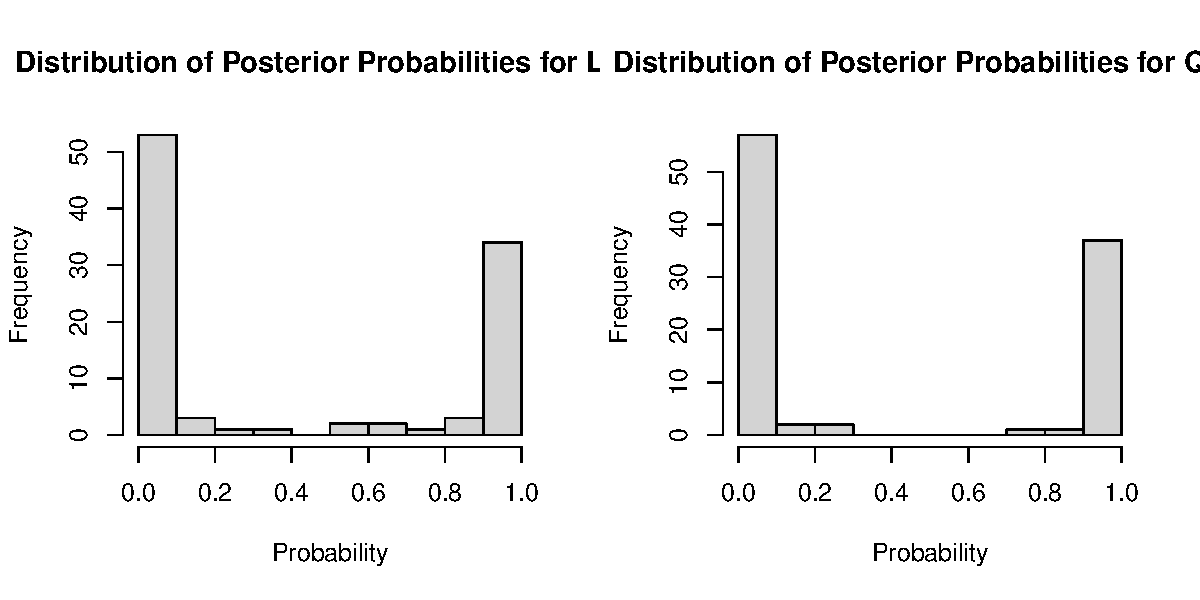
\includegraphics{me_files/figure-pdf/Distribution of Posterior-1.pdf}

}

\caption{Distribution of Posterior Probabilities}

\end{figure}%

\subsection{nn work}\label{nn-work}

Neural networks improve predictive performance by capturing complex
nonlinear relationships between features and the target variable. With
multiple hidden layers and structured activation functions, they learn
intricate patterns in the data. Additionally, their architecture reduces
dependence on any single feature, enhancing generalization.

Based on the PCA results, we initially designed a neural network with
two hidden layers: the first layer containing 47 neurons and the second
layer containing 20 neurons. This structure was chosen to capture the
primary features of the dataset while maintaining a balance between
model complexity and computational efficiency. The aim was to leverage
the dimensionality reduction insights from PCA to guide the architecture
design and improve the model's ability to extract meaningful patterns
from the data.

The training performance was suboptimal, and the model did not meet
expectations. One possible reason for this was the insufficient network
capacity, which prevented the model from fully capturing the complex
patterns within the data.

\#\#Adjustment Strategy To improve the model's learning ability, we
increased the number of neurons in the first hidden layer to 533,
enhancing its capability to extract meaningful features. In the
subsequent hidden layers, we gradually reduced the number of neurons to
256 → 60 → 20, aiming to refine the model's representation while
preventing overfitting. This hierarchical structure allows the network
to capture high-dimensional features in the initial layers and
progressively distill the most relevant information in the deeper
layers.

The training performance improved significantly, with the AUC increasing
from 0.64 to 0.95. This dramatic improvement suggests that the adjusted
network architecture effectively enhanced the model's ability to learn
complex patterns, leading to a much better classification performance.
The increased network capacity in the initial layers allowed for better
feature extraction, while the gradual reduction in neurons helped refine
the representations, ultimately resulting in a more robust and
well-generalized model.

\begin{figure}[H]

{\centering 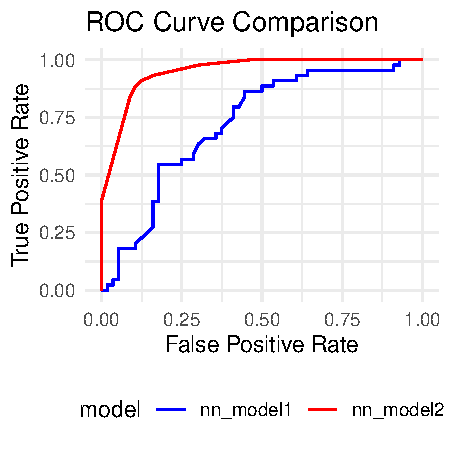
\includegraphics{me_files/figure-pdf/nnROC-1.pdf}

}

\caption{ROC of nn1 and nn2}

\end{figure}%

\subsection{SVM}\label{svm}

The datasets contain features derived from different preprocessing
methods:

\begin{itemize}
\item
  Dataset 1: Original dataset with 5000 features.
\item
  Dataset 2: Feature selection reduced the number of features to 1824.
\item
  Dataset 3: Principal Component Analysis (PCA) reduced the feature
  count to 47.
\end{itemize}

For each dataset, SVM models were trained, tested, and optimized using
GridSearchCV to identify the best hyperparameters. The datasets were
loaded and divided into features (X) and target labels (y).
Standardization was applied using StandardScaler to ensure the SVM
operates effectively. An initial SVM model with default parameters was
trained on each dataset. Model performance was evaluated using accuracy
and Area Under the Curve (AUC) scores. Hyperparameter tuning was
performed using GridSearchCV to optimize SVM parameters (C, gamma, and
kernel). The best model from the grid search was selected and evaluated
on the test set. The following hyperparameters were explored: C:
{[}0.01, 0.1, 0.5, 1, 2, 10, 100{]}, gamma: {[}``scale'', ``auto'',
0.01, 0.1, 1{]}, kernel: {[}``linear'', ``rbf'', ``poly''{]}. The best
hyperparameters were selected based on AUC scores.

\begin{longtable}[]{@{}llll@{}}
\toprule\noalign{}
Dataset & Features & Accuracy & AUC \\
\midrule\noalign{}
\endhead
\bottomrule\noalign{}
\endlastfoot
Original & 5000 & 0.84 & 0.930 \\
Feature selection & 1824 & 0.88 & 0.948 \\
PCA Reduction & 47 & 0.81 & 0.924 \\
\end{longtable}

\begin{verbatim}
# A tibble: 1 x 7
  format width height colorspace matte filesize density
  <chr>  <int>  <int> <chr>      <lgl>    <int> <chr>  
1 PNG     1282    452 sRGB       TRUE         0 87x87  
\end{verbatim}

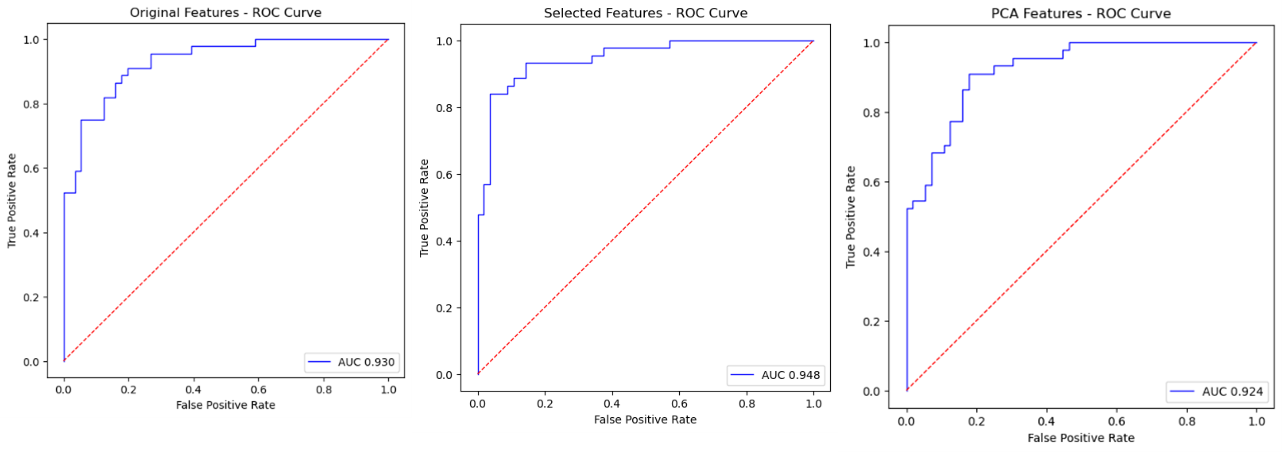
\includegraphics[width=4.27in,height=\textheight]{me_files/figure-pdf/unnamed-chunk-31-1.png}

Reducing the number of features from 5000 to 1824 improved accuracy and
AUC after tuning. PCA-reduced data (47 features) maintained good
accuracy but performed slightly worse than feature selection. In most
cases, GridSearchCV improved AUC over the default model. For Dataset 1,
a linear kernel was chosen as optimal, while for Datasets 2 and 3, an
RBF kernel was preferred.~ ~

Feature selection (1800 features) provided the best performance in terms
of both accuracy and AUC. PCA (40 features) led to minor accuracy
reduction but is still a viable option for dimensionality reduction.




\end{document}
